% This is LLNCS.DEM the demonstration file of
% the LaTeX macro package from Springer-Verlag
% for Lecture Notes in Computer Science,
% version 2.3 for LaTeX2e



\documentclass{llncs}


\usepackage{ngerman}
\usepackage[T1]{fontenc}
\usepackage[utf8]{inputenc}
\usepackage{makeidx}  % allows for indexgeneration
\usepackage{multirow}
\usepackage{rotating}
\usepackage{verbatim}
\usepackage{graphicx}
\usepackage{float}
\usepackage{amssymb}   % AMS-Sonderzeichen
\usepackage{tabularx}  % Für tabularx und newcolumntype
\usepackage[paper=a4paper,left=25mm,right=25mm,top=25mm,bottom=25mm]{geometry}
\usepackage{array}
\usepackage{makecell}
\usepackage{color}
\usepackage{ragged2e}
\usepackage{ifpdf}
% \usepackage{titlesec}
\usepackage{xcolor}    % Lieber xcolor als color. Dann klappt auch das listings gut mit den Farben
\usepackage{listings}
\usepackage{upquote}   % Verändert die Ausgabe der einfachen Anführungszeichen innerhalb von verbatim
\usepackage{eurosym}   % Euro-Zeichen: \euro
\usepackage{lastpage}  % \pageref{LastPage} um die Anzahl der Seiten zu erhalten
% hiermit kann man auch umlaute copy-pasten
\usepackage{lmodern}
\selectlanguage{english}
\usepackage{fancyhdr}
\usepackage{url}
\usepackage{caption}
\usepackage{float}
\setlength{\abovecaptionskip}{0pt} % Reduce space above the caption
\setlength{\belowcaptionskip}{0pt} % Space between caption and table
\captionsetup[table]{skip=5pt} % Adjust the value of '10pt' as needed
\pagestyle{fancy}
% Reduce space between float and surrounding text
\setlength{\textfloatsep}{0pt}
\setlength{\floatsep}{0pt}
\setlength{\intextsep}{0pt}



%

\ifpdf
\pdfinfo{
   /Author (Wladymir Alexander Brborich Herrera)
   /Author (Vishwaben Pareshbhai Kakadiya)
   /Author (Hellyben Bhaveshkumar Shah)
   /Author (Heer Rakeshkumar Vankawala)
   /Author (Priyanka Dilipbhai Vadiwala)
   /Title  (LowTech GMmBH Techincal Transformation Milestone 1)
   /Subject (Cloud Computing)
   /Keywords (Cloud Computing, Technical Transformation, Migration)
}
\fi

\setlength{\parindent}{0pt}    % Erste Zeile eines Absatzes nicht einrücken
\parskip2ex                    % Absatzabstand
\setlength{\itemsep}{0ex plus0.2ex}
\sloppy                        % Auf jeden Fall die Seitenränder einhalten.

\newcommand{\what}{Milestone 1 : LowTech GMmBH Techincal Transformation on Premises}
\newcommand{\who}{Group 23}
\newcommand{\when}{WiSe 2024-2025}

\renewcommand{\headrulewidth}{0.4pt}
\renewcommand{\footrulewidth}{0.4pt}
\lhead[\when]{\who}
\rhead[\who]{\when}
\chead[]{}
\lfoot[Page \thepage\ of \pageref{LastPage}]{\what}
\rfoot[\what]{Page \thepage\ of \pageref{LastPage}}
\cfoot[]{}
\pagestyle{fancy}


% Hurenkinder und Schusterjungen komplett verbieten.
\clubpenalty = 10000 
\widowpenalty = 10000 
\displaywidowpenalty = 10000
% Diese Begriffe bezeichnen den Makel beim Textsatz, wenn eine Seite mit der ersten Zeile eines Absatzes endet (so genannter Schusterjunge) oder eine neue Seite mit der letzten Zeile eines Absatzes beginnt (so genanntes Hurenkind).


% Wir definieren ein paar Farben
\definecolor{Brown}{cmyk}{0,0.81,1,0.60}
\definecolor{OliveGreen}{cmyk}{0.64,0,0.95,0.40}
\definecolor{CadetBlue}{cmyk}{0.62,0.57,0.23,0}
\definecolor{lightlightgray}{gray}{0.9}
\definecolor{FrankfurtBlue}{HTML}{3333b2}

% Hier fängt das Dokument an!
\begin{document}

%
% \frontmatter          % for the preliminaries
%
% \tableofcontents
%
\mainmatter              % start of the contributions
%
\title{\what}
%
\author{
  Wladymir Alexander Brborich Herrera\\
  \texttt{wladymir.brborich-herrera@stud.fra-uas.de}
  \and\\ 
  Vishwaben Pareshbhai Kakadiya (1471845)\\
  \texttt{vishwaben.kakadiya@stud.fra-uas.de}
  \and\\
  Hellyben Bhaveshkumar Shah (1476905)\\
  \texttt{hellyben.shah@stud.fra-uas.de}
  \and\\
  Heer Rakeshkumar Vankawala (1449039)
  \\
  \texttt{heer.vankawala@stud.fra-uas.de}
  \and\\
  Priyanka Dilipbhai Vadiwala (1481466)\\
  \texttt{priyanka.vadiwala@stud.fra-uas.de}
}
%
\institute{
  Frankfurt University of Applied Sciences\\
  (1971-2014: Fachhochschule Frankfurt am Main)\\
  Nibelungenplatz 1\\
  D-60318 Frankfurt am Main\\
}

\maketitle              % typeset the title of the contribution

\begin{abstract}
  In this report, we as consultants from \textit{Awesome Cloud AG} present a technical transformation analysis aimed at modernizing the infrastructure of \textit{LowTech GmbH}, 
  a small to medium-sized enterprise specializing in wooden furniture production. 
  The analysis includes a critical assessment of the current infrastructure, energy consumption calculation for the existing setup 
  followed by a detailed transformation roadmap of future-ready modern infrastructure and explanations of enhancements in scalability, availability, and security compared to current infrastructure. 
  This analysis will serve as a foundational step for subsequent project phases, ensuring that \textit{LowTech GmbH} is well-equipped to meet future requirements and challenges.
\end{abstract}

\section{Overview of the Problem}

LowTech GmbH, a small to medium-sized enterprise with 45 employees specializing in wooden furniture production, is facing a critical need for technological transformation. 
Initially relying on sales representatives, the company transitioned to an online store a few years ago, which has now become their primary selling platform. 
This shift has led to a significant increase in user numbers over the past two years, necessitating a modernization of their IT infrastructure. 
The CEO of LowTech GmbH, recognizing the need for modernization, has expressed interest in cloud computing to make the company future-ready.

\section{Objectives of the Technological Transformation}

The objective of the technological transformation for LowTech GmbH is to modernize its server and application infrastructure by migrating to a private cloud environment. 
This initiative aims to create a scalable, secure, and efficient IT framework that aligns with the company's growing needs, particularly in response to increased online sales and user traffic. 
By adopting a private cloud strategy, LowTech GmbH will retain control over its data while outsourcing hardware maintenance to a third-party provider. 
This transition will involve leveraging newer technologies to enhance performance and availability, ensuring compliance with security standards, and reducing operational costs. 
Ultimately, the transformation seeks to provide a future-ready infrastructure that supports the company's evolving business model and operational requirements.

\section{Assessment of the Current (as-is) Infrastructure}

\subsection{Scalability, Availability and Security Analysis}
According to NIST definition of cloud computing is given as ``Cloud computing is a model for enabling ubiquitous, convenient, on-demand network access to a shared
pool of configurable computing resources (e.g., networks, servers, storage, applications, and services) that
can be rapidly provisioned and released with minimal management effort or service provider interaction.'' \cite{mell2011nist}

As \textit{LowTech GmbH} is based on Legacy IT infrastructure and currently lacking \textit{NIST five
  essential characteristics} such as On-demand self-service, Broad network access,Resource pooling,Rapid elasticity and Measured service.

\subsubsection*{Elasticity / Scalability}

\begin{itemize}
  \item \textbf{Fixed Hardware \& Inflexible Infrastructure}:
        \\
        Current infrastructure consists of 7 on-premises servers housed in a single 19-inch rack, 
        along with 17 clients and 19 laptops all with predetermined, static configurations. 
        Moreover, the physical constraints of the on-premises setup, with no additional space for expansion, severely limit scaling options. 
        This inflexibility makes it challenging to accommodate growth or adapt to changing business needs.
        \\
  \item \textbf{Absence of Resource Utilization/pooling}:
        \\ 
        There's no apparent way to quickly scale resources up or down based on demand or user traffic fluctuation in the current infrastructure. 
        Each application typically runs on a dedicated server with fixed resources. 
        This approach leads to inefficient resource utilization, as some servers may be underutilized while others are overloaded which may lead to performance issues during peak times or resource waste during low-demand periods due to no dynamic resource allocation.
        \\
  \item \textbf{Manual Processes \& High Cost}:
        \\ 
        Any changes in capacity would likely require manual hardware upgrades or replacements including hardware installation,
        and configuration, making the process time-consuming and potentially leading to downtime.
        Replacement of hardware is not only tedious but also financially burdensome due to high costs of new hardware.
        
\end{itemize}

\subsubsection*{Availability}
\begin{itemize}
  \item \textbf{Obsolete Hardware/OS \& Runtime Environments}:
        \\
        Many components of the current infrastructure is based on very old hardware and outdated operating systems such as 
        Windows XP SP3 (Finance clients), Windows 7 SP3 (HR clients and Customer Service laptops), Debian 5.0 Lenny (Warehouse clients and server),
        Ubuntu 16.04 LTS (Sales CRM Storage server) etc. Several applications are running on outdated software versions such as Java 1.7/1.8, 
        MySQL 5.5/5.7, PHP 5.3 and Firefox 3.6 etc. which makes this whole infrastructure more susceptible to failure.
        \\
  \item \textbf{Lack of Redundancy and Backup Mechanism}:
        \\ 
        There's no mention of redundant systems or data backup solutions which might lead to significant service disruptions as well as data loss in case of any system failure.
        \\
  \item \textbf{Manual Maintainance}:
        \\It is impossible to meet high availability requirements without a robust failover mechanism due to manual maintenance operations. 
        This increases the possiblity of human errors, leads to longer downtime and reduces overall reliability.
        \\
\end{itemize}

\subsubsection*{Security}
\begin{itemize}
  \item \textbf{Basic Windows Firewall}:
        \\
        It provides minimal outward traffic control, which may allow malware to interact easily. 
        Without additional tools, centralized administration is impossible to maintain consistent security rules across all 36 client devices (17 clients and 19 laptops).
        It lacks advanced threat protection features, leaving the system vulnerable to sophisticated attacks.
        \\
  \item \textbf{pfSense for Network Packet Filtering}:
        \\ 
        There are no built-in antivirus features, which could let malicious payloads get through. Its effectiveness heavily relies on proper configuration, which may be challenging without dedicated IT staff.
        Moreover, advanced intrusion detection requires additional setup and maintenance.
        \\
        
\end{itemize}
This can harm company's overall reputations due to risk of potential data breaches followed by financial loss, legal implications as well as loss of customer's trust.
\subsection{Energy Consumption and Approximate Cost}

Energy consumption calculation for the as-in infrastructure of Low Tech GmbH is as follows : 

\begin{table}[htbp]
  \centering
  \begin{tabular}{|l|c|c|c|c|c|}
    \hline
    \textbf{Departments} & \textbf{Server}          & \textbf{Client}          & \textbf{Laptop}          & \textbf{Total Power}   & \textbf{Annual Energy}      \\
                         & \textbf{ (Qty x Power) } & \textbf{ (Qty x Power) } & \textbf{ (Qty x Power) } & \textbf{ Consumption } & \textbf{ Consumption(KWh) } \\
    \hline
    Finance              & 1 x 1000W                & 4 x 500W                 & -                        & 3000W                  & 26,280                      \\
    \hline
    HR                   & 1 x 1000W                & 3 x 500W                 & -                        & 2500W                  & 21,900                      \\
    \hline
    Warehouse            & 1 x 1000W                & 10 x 500W                & -                        & 6000W                  & 52,560                      \\
    \hline
    Sales                & \makecell{1 x 1000W                                                                                                                   \\ 1 x 1200W} & - & 10 x 50W & 2700W & 23,652 \\
    \hline
    Operations           & 1 x 1200W                & -                        & 4 x 50W                  & 1400W                  & 12,264                      \\
    \hline
    Customer Service     & -                        & -                        & 5 x 100W                 & 500W                   & 4,380                       \\
    \hline
    Webshop              & 1 x 1200W                & -                        & -                        & 1200W                  & 10,512                      \\
    \hline
  \end{tabular}
  \caption{Power Consumption by Department and Device Type}
  \label{tab:power_consumption}
\end{table}

\textbf{Total Energy Consumption (Annual)} : 151,548 KWh (151.548 MWh)

According to Eurostat published data of electricity prices for non-household consumers \cite{eurostat2023}, Low Tech GmbH falls under the annual energy consumption band 
`IB (20 MWh to 499 MWh)' with energy price 0.3244 \EUR{} per KWh.


\textbf{Total Cost for Energy Consumption (Annual)} : 151,548 KWh x 0.3244 \EUR{} = 49,162.17 \EUR{}

\section{Client Requirements}

\begin{itemize}
  \item Make the infrastructure more scalable, available and secure
  \item Modernize the technology, runtime and operation modality
  \item Perform the migration with a maximum downtime of 4 hours
  \item Cost reduction
  \item Maintenance reduction
  \item High availability of 99.5\%
\end{itemize}

\section{Assessment of Potential Technological Components}

\subsection{Hardware}
\vspace{-10pt}
\begin{table}[H]
  \setlength{\tabcolsep}{5pt} % Adjust column spacing
  \renewcommand{\arraystretch}{1.2} % Adjust row spacing
  \centering
  \begin{tabular}{|p{3cm}|p{8cm}|p{4cm}|}
  \hline
  \textbf{Component} & \textbf{Details} & \textbf{Options} \\
  \hline
  \textbf{Compute and Storage} & 
  A hyper-converged infrastructure (HCI) combining compute, storage, and networking in a single system. & 
  \textbf{Primary Options:} \newline 
  - Dell VxRail \newline 
  - Nutanix NX-Series \newline 
  \textbf{Alternative:} \newline 
  - HPE ProLiant DX series \\
  \hline
  \textbf{Form Factor} & 
  1U to 2U rack-mounted nodes that fit into a 19-inch rack. & 
  \\
  \hline
  \textbf{Capabilities} & 
  High-density storage and compute with built-in redundancy; supports scaling and maintenance. & 
  \\
  \hline
  \textbf{Features} & 
  Virtualization, software-defined storage (SDS), integrated backup, and disaster recovery. & 
  \\
  \hline
  \textbf{Storage Options} & 
  & 
  \\
  \hline
  \textbf{All-Flash Array} & 
  High I/O performance for databases like CRM and Payroll. & 
  - Pure Storage FlashArray \newline 
  - Dell EMC PowerStore \\
  \hline
  \textbf{Hybrid Storage} & 
  Mix of SSDs and HDDs to balance performance and cost. & 
  SSDs for frequently accessed data; HDDs for less critical storage needs. \\
  \hline
  \textbf{Backup Appliance} & 
  Dedicated appliance for securing backups and enabling data restoration. & 
  - Dell EMC Data Domain \newline 
  - HPE StoreOnce \\
  \hline
  \end{tabular}
  \caption{Overview of Components and Options}
  \label{tab:components}
  \end{table}  

\subsection{Virtualization and Hypervisor technologies}
\vspace{-10pt}
\begin{table}[H]
  \setlength{\tabcolsep}{5pt} % Adjust column spacing
  \renewcommand{\arraystretch}{1.2} % Adjust row spacing
  \centering
  \begin{tabular}{|p{3.5cm}|p{7cm}|p{4.5cm}|}
  \hline
  \textbf{Technology} & \textbf{Features} & \textbf{Advantages/Options} \\
  \hline
  
  \textbf{VMware vSphere} & 
  Industry-standard hypervisor with advanced features: \newline 
  - High availability (HA) \newline 
  - vMotion (for live migrations) \newline 
  - Distributed Resource Scheduling (DRS). & 
  Well-suited for HCI setups. \newline 
  Granular control and easy integration with VMware products such as: \newline 
  - vSAN (for storage) \newline 
  - NSX (for networking). \\
  \hline
  
  \textbf{Microsoft Hyper-V on Windows Server 2022} & 
  Features: \newline 
  - Replication \newline 
  - Clustering \newline 
  - Live migration. & 
  Cost-effective and works well with Microsoft environments. \newline 
  Ideal if LowTech GmbH uses Microsoft products. \newline 
  Supports containers and VMs in the same environment. \\
  \hline
  
  \textbf{Management Tool} & 
  Centralized management, monitoring, and configuration of virtualized resources. & 
  Options: \newline 
  - VMware vCenter \newline 
  - Microsoft System Center \\
  \hline
  
  \textbf{Containerization Platform} & 
  Use Kubernetes for managing and orchestrating containers for applications. \newline 
  Suitable for containerized apps like microservices for webshop or CRM. \newline 
  Provides flexibility for hybrid cloud migration and easy scaling. & 
  Options: \newline 
  - VMware Tanzu \newline 
  - Red Hat OpenShift \\
  \hline
  
  \end{tabular}
  \caption{Comparison of Technologies and Features}
  \label{tab:technologies}
  \end{table}
  
\subsection{Firewall and Network Security}
\begin{table}[H]
  \setlength{\tabcolsep}{5pt} % Adjust column spacing
  \renewcommand{\arraystretch}{1.2} % Adjust row spacing
  \centering
  \begin{tabular}{|p{3cm}|p{7cm}|p{5cm}|}
  \hline
  \textbf{Technology} & \textbf{Features} & \textbf{Advantages} \\
  \hline
  
  \textbf{Firewall} & 
  Next-Generation Firewall (NGFW): Fortinet FortiGate or Palo Alto Networks PA-Series. \newline 
  \textbf{Capabilities:} Packet filtering, intrusion prevention, VPN, application control, and threat intelligence. & 
  Provides both perimeter and internal segmentation security, which is crucial for sensitive data in CRM and payroll applications. \\
  \hline
  
  & pfSense (Advanced Version): Open-source firewall/router solution with load balancing, failover, and VPN. & 
  Cost-effective and highly configurable. Suitable for tighter budgets but lacks enterprise-grade features like FortiGate or Palo Alto. \\
  \hline
  
  \textbf{Intrusion Detection/Prevention System (IDS/IPS)} & 
  Suricata or Snort (for pfSense): Open-source IDS/IPS options that integrate with pfSense. & 
  Popular open-source options for network intrusion detection and prevention. \\
  \hline
  
  & Cisco Firepower or FortiGate Intrusion Prevention (if using Fortinet or Palo Alto NGFW): Integrated network threat protection. & 
  Integrated with NGFWs for enhanced threat detection and prevention. \\
  \hline
  
  \textbf{Network Segmentation} & 
  Use VLANs and/or virtual firewalls to isolate sensitive areas of the network (e.g., HR, Finance, and CRM databases). & 
  Helps protect critical data by isolating sensitive areas from the public-facing webshop. \\
  \hline
  
  \end{tabular}
  \caption{Network Security Technologies and Their Advantages}
  \label{tab:network_security}
  \end{table}
  
\subsection{Backup and Disaster Recovery}
\begin{table}[H]
  \setlength{\tabcolsep}{5pt} % Adjust column spacing
  \renewcommand{\arraystretch}{1.2} % Adjust row spacing
  \centering
  \begin{tabular}{|p{3cm}|p{7cm}|p{5cm}|}
  \hline
  \textbf{Solution} & \textbf{Features} & \textbf{Advantages} \\
  \hline
  
  \textbf{Backup Solution} & 
  Veeam Backup \& Replication: Provides comprehensive backup, recovery, and replication for virtual machines, containers, and physical servers. & 
  Easy integration with VMware and Hyper-V. Supports off-site backups to cloud services and ensures rapid recovery times. \\
  \hline
  
  & Commvault Complete Data Protection: A scalable backup solution for large-scale environments. & 
  Offers similar features to Veeam with more granular data management. \\
  \hline
  
  \textbf{Disaster Recovery (DR)} & 
  Zerto: Real-time replication and disaster recovery capabilities. Can replicate VMs between on-premises and cloud environments. & 
  Enables a future hybrid setup with minimal downtime. \\
  \hline
  
  & VMware Site Recovery Manager (SRM): Automatic failover and failback of VMs in VMware environments. & 
  Tailored for VMware setups; streamlines disaster recovery processes. \\
  \hline
  
  \end{tabular}
  \caption{Backup and Disaster Recovery Solutions}
  \label{tab:backup_dr}
  \end{table}

\subsection{Software Components}

\begin{table}[H]
\setlength{\tabcolsep}{5pt} % Adjust column spacing
\renewcommand{\arraystretch}{1.2} % Adjust row spacing
\centering
\begin{tabular}{|p{4cm}|p{6cm}|p{5cm}|}
\hline
\textbf{Category} & \textbf{Features} & \textbf{Advantages/Options} \\
\hline

\textbf{Configuration Management} & 
Ansible: Automates configuration and deployment of applications across servers. Uses playbooks to simplify repetitive tasks. &
Reduces maintenance efforts and ensures consistency across servers. \\
\hline

\textbf{DevOps Tools} & 
GitLab or Jenkins: Tools for CI/CD (Continuous Integration/Continuous Deployment) pipelines. Automates testing and deployment processes. &
Improves agility and reduces downtime by streamlining application updates. \\
\hline

\textbf{VPN and Remote Access} & 
OpenVPN or Fortinet VPN: Provides secure remote access. Enable multi-factor authentication (MFA) for enhanced security. &
Ensures secure connectivity for remote users while protecting sensitive systems. \\
\hline

\end{tabular}
\caption{Other Software Components}
\label{tab:software_components}
\end{table}
\section{Migration to a Private-Cloud Context}

To perform a successful migration to a private cloud context we have analyzed the baseline performance of the current system, as well as the technologies used. Based on the client requirements, we have selected technologies and established a roadmap to perform this task.   

\subsection{Architecture}

\begin{figure}[htbp]
  \begin{center}
    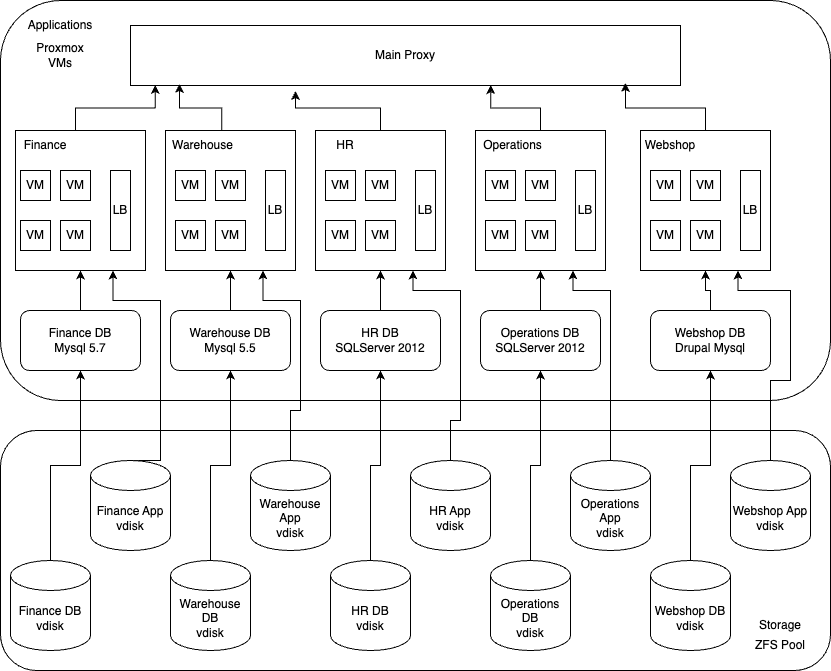
\includegraphics[width=11cm]{diagrams/architecture.drawio.png}
    \caption{High Level Architecture~\ref{High_Level_Architecture}}
    \label{High_Level_Architecture} % A unique label.
  \end{center}
\end{figure}

Note: We could use one VM and Docker to run most of the database instances as containers, making it easier to install or upgrade versions. Nevertheless, some of the tools are difficult to dockerize (SQLServer 2012) and, we want to have isolation between departments, preventing a single point of failure for all our database infrastructure.

\begin{figure}[htbp]
  \begin{center}
    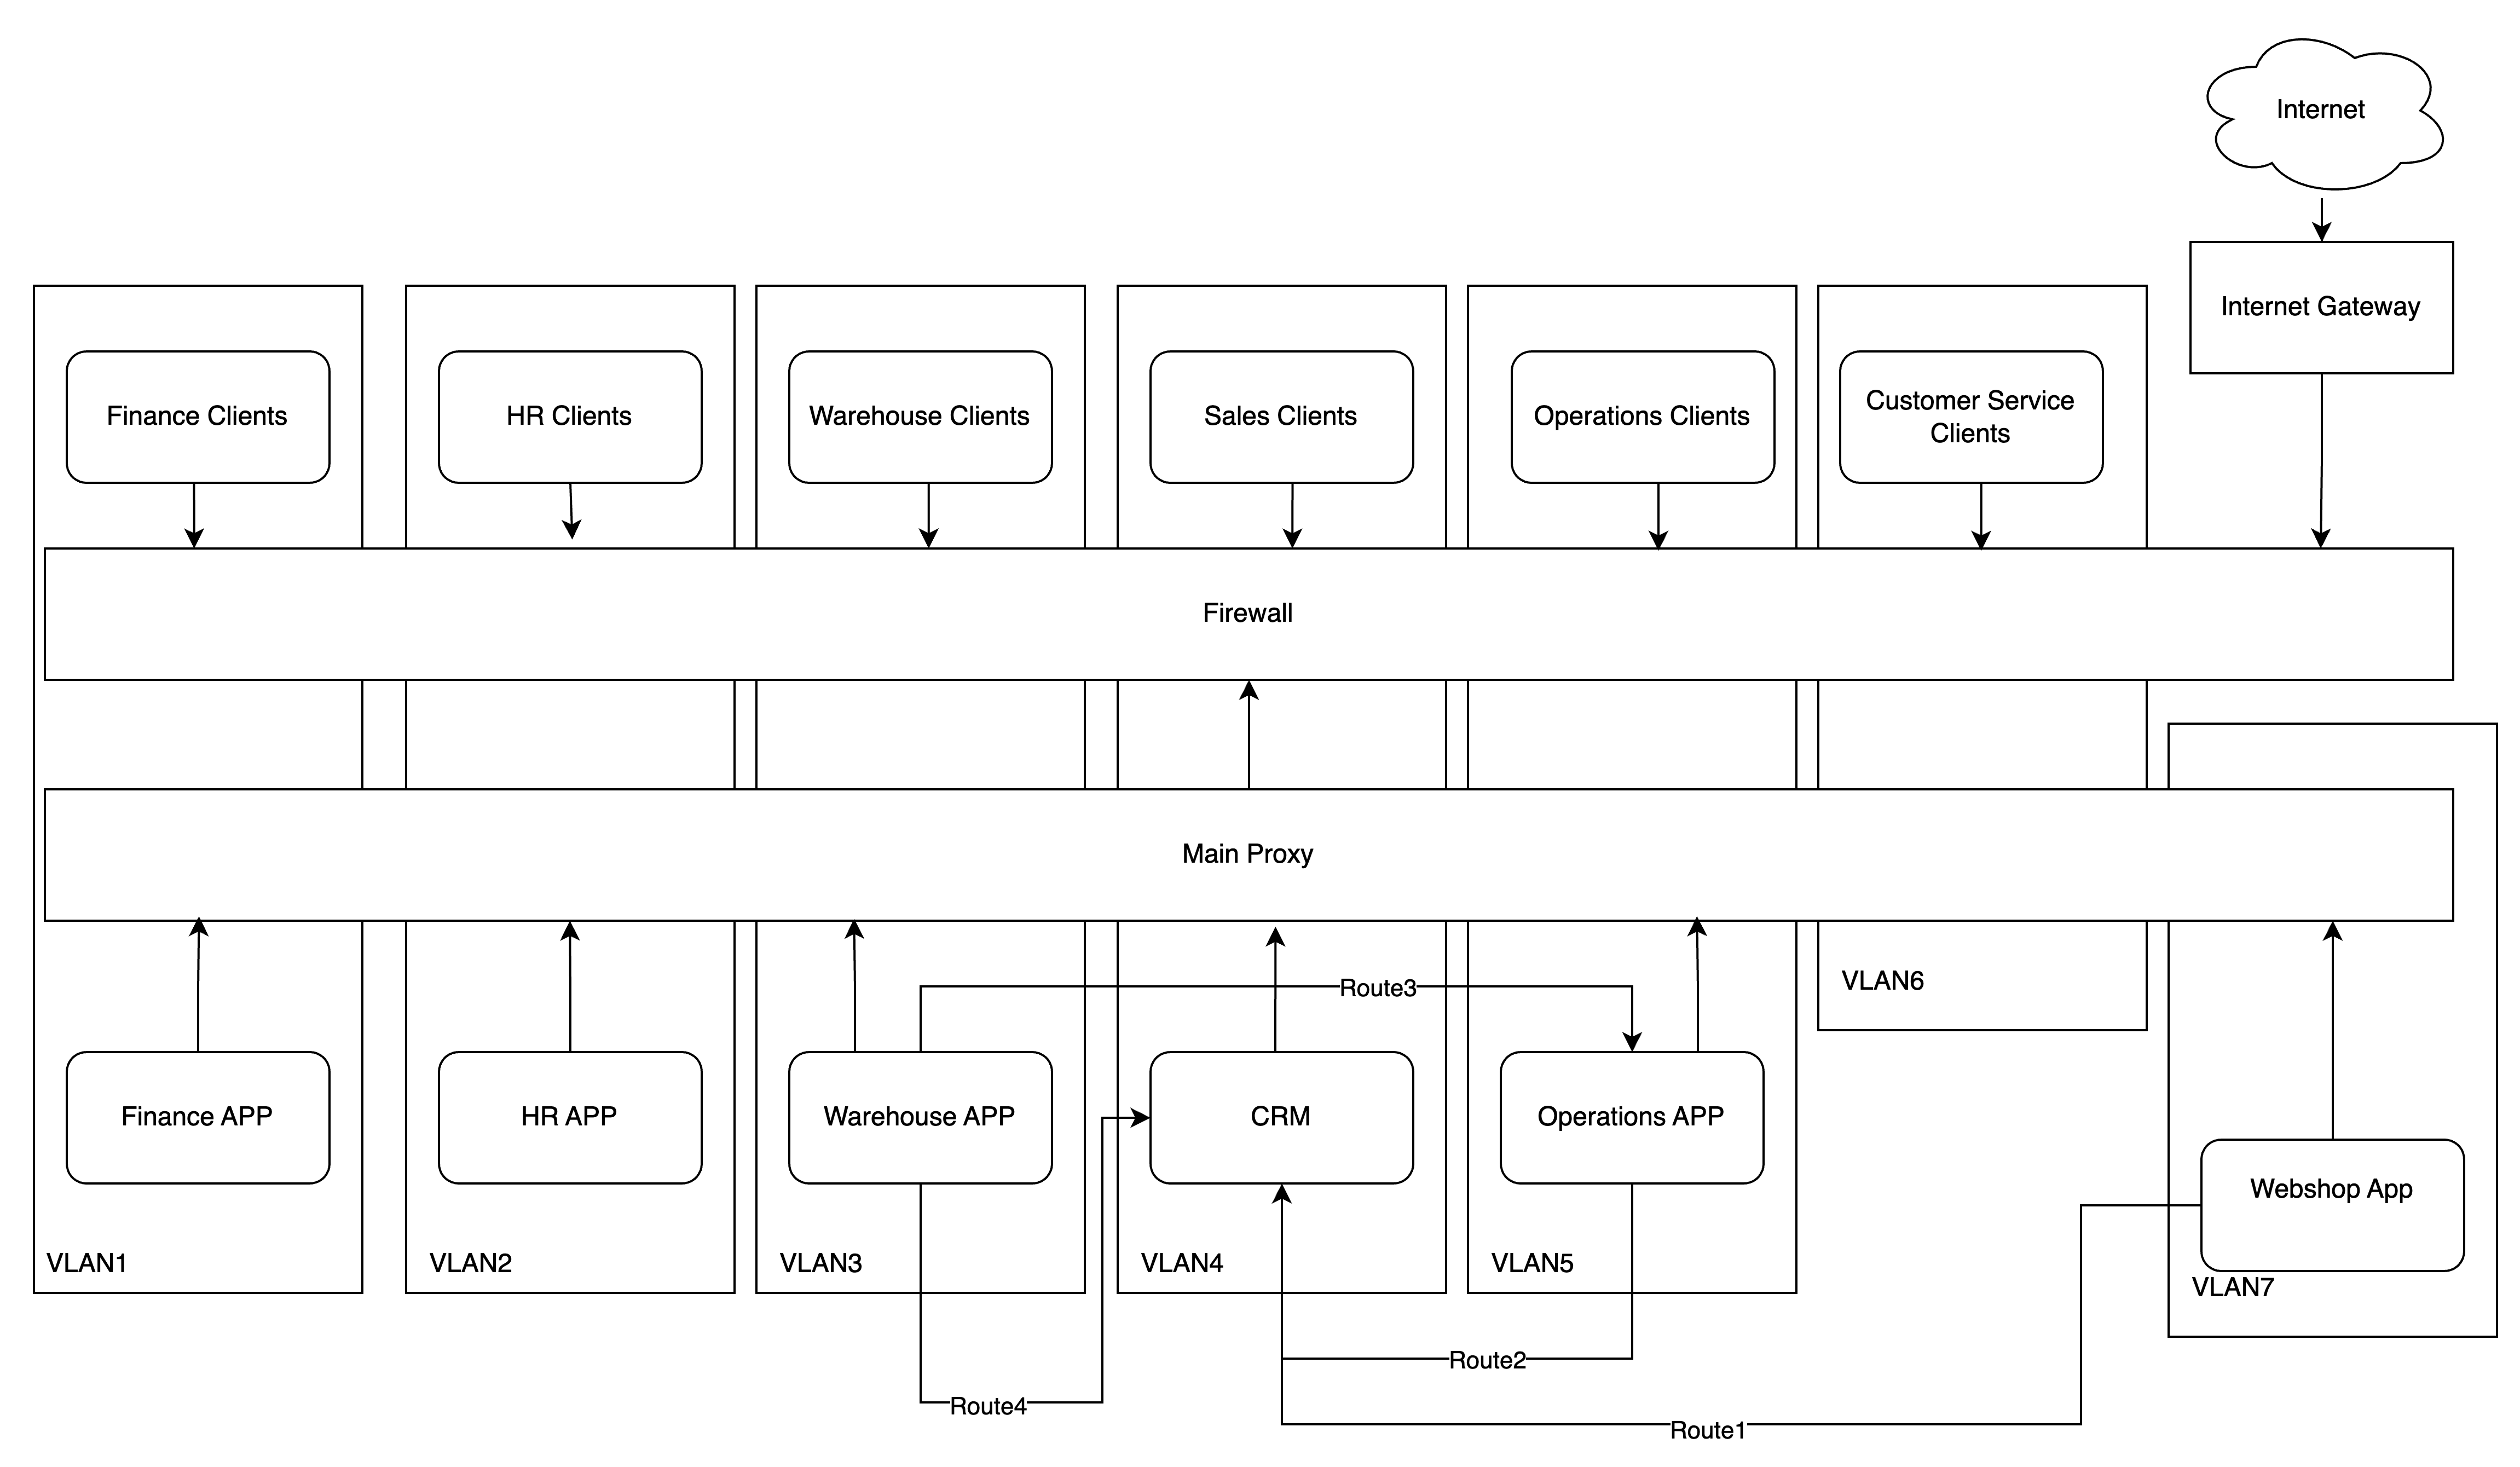
\includegraphics[width=11cm]{diagrams/network_architecture.png}
    \caption{Network Architecture~\ref{Network_Architecture}}
    \label{Network_Architecture} % A unique label.
  \end{center}
\end{figure}

We subdivide each department into its own network, virtually limiting the access of different clients to their corresponding systems. And only systems can have cross department routes to stablish communication for normal operation. 

\section{Roadmap}

The technological transformation roadmap is divided in four phases: Assessment, Design, Execution, and Optimization.

\subsection{Assessment}
This is the most critical step. We need to establish a baseline of performance, and cost of the current infrastructure. During this stage we are going to execute the following tasks:

\begin{itemize}

  \item Review the current infrastructure in terms of performance, data requirements, availability and security. Establishing baseline metrics we then have some rough idea of the areas we want to pay attention, and  at the end, the total impact that the migration had. We have some rough figures provided by the client, but these are not enough to actually guide development.
  \item Check the current applications, to define a migration approach, if they can be migrated, changed, or improved in a way that makes the transition process easier. Given the initial requirements, we can assume that the applications are not actively being developed, so modernization is not an approach we can consider at that level.
  \item Identify the level of effort per department/application/domain to make the migration, this metrics will guide the order of the execution. This is to reduce the impact of the migration in the business operation. Naturally there will be usage patterns more friendly to upgrade and intervention.
  \item Assess the budget and space constraints for new hardware, or to rent such services. A preliminary review points to renting server space as the most appropriate solution. To achieve the availability metrics required by the customer will require a great investment in provisioning, modernizing and validating the current server location. Not only in technological terms, but also: physical security, thermal management, internet bandwidth and energy provisioning.
  \item Spec the hardware after evaluating the usage pattern and metrics. We want to, not only get parity to the current hardware but have space to grow.
\end{itemize}
\subsubsection{Rental Cost Calculation}
\textbf{Option 1: Cloud Rental (Monthly Cost Calculation)}
\vspace{3pt}
\begin{table}[H]
\centering
\begin{tabular}{|>{\raggedright\arraybackslash}p{3cm}|>{\raggedright\arraybackslash}p{6cm}|>{\raggedleft\arraybackslash}p{3cm}|>{\raggedleft\arraybackslash}p{3cm}|}
\hline
\textbf{Component}      & \textbf{Quantity/Details}                          & \textbf{Unit Cost} & \textbf{Total Cost} \\ \hline
Compute (VMs)           & 12 Medium VMs (8 vCPUs, 32GB RAM, 1TB SSD)         & \$300 per VM/month & \$3,600             \\ \hline
Storage                 & 6TB Cloud Storage (e.g., Amazon S3/Glacier)        & \$20 per TB/month  & \$120               \\ \hline
Bandwidth               & 500GB (9000 visits, 250KB payload each)            & \$0.15 per GB      & \$75                \\ \hline
\textbf{Total Cloud Rental Cost} &                                          &                    & \textbf{\$3,795/month} \\ \hline
\end{tabular}
\caption{Cloud Rental Cost Breakdown}
\end{table}

\textbf{Option 2: Dedicated Rental (Monthly Cost Calculation)}
\vspace{3pt}
\begin{table}[h!]
\centering
\begin{tabular}{|>{\raggedright\arraybackslash}p{3cm}|>{\raggedright\arraybackslash}p{6cm}|>{\raggedleft\arraybackslash}p{3cm}|>{\raggedleft\arraybackslash}p{3cm}|}
\hline
\textbf{Component}      & \textbf{Quantity/Details}                          & \textbf{Unit Cost} & \textbf{Total Cost} \\ \hline
Dedicated Servers       & 6 Servers (32 vCPUs, 128GB RAM, 2TB SSD)           & \$750 per Server/month & \$4,500         \\ \hline
Storage                 & 6TB SAN/NAS Storage for CRM and Sales data         & \$125 per TB/month & \$750               \\ \hline
Bandwidth               & Included in Dedicated Hosting                      & \$0                & \$0                 \\ \hline
\textbf{Total Dedicated Rental Cost} &                                       &                    & \textbf{\$5,250/month} \\ \hline
\end{tabular}
\caption{Dedicated Rental Cost Breakdown}
\end{table}

\subsection{Design}

In this step we perform the following tasks:

\begin{itemize}

  \item Design the new architecture diagram with networking isolation between domains, dividing each department appropriately.
  \item Document which applications will be migrated to new technologies, or will be ported as is.
  \item Create document with detailing the dates and approximate duration of the migration each application. This is to be distributed to the organization so operation disruption is minimized
  \item Prepare contingency plans, and fallbacks to minimize disruption to the business if a migration fails. This could take the form of rollbacks, traffic duplication or A/B testing. Depending on the need of each department and the complexity of each application
  \item Create all the technical documentation regarding the implementation for the application migrations to new technologies.
\end{itemize}

\subsection{Execution}

In this step we perform the following tasks:
\begin{itemize}

  \item  Talk with server space providers, we need to stablish a contract and negotiate price and SLOs based on the server requirements
  \item Gather all the installation information, binaries, licenses and documentation for all applications.
  \item Configure a development environment to upload all artifacts such as configuration files and container images.
  \item Create Ansible configuration files for each application, to automate the installation and replication process.
  \item Develop scripts to automate application functionality and load testing. To determine if the configurations will be on par or better than the current infrastructure.
  \item Provision and install the private cloud management software, including the networking configuration
  \item Configure the storage
  \item Create the virtual machines for the base hosts
  \item Configure Prometheus to monitor the virtual machine installations
  \item Establish the network links between the different virtual domains
  \item Install all database servers
  \item Develop a migration process to replicate the current data into the new database servers.
  \item Review that data is up to parity with the legacy services
  \item Create a proxy getaway for the services, so we can redirect the traffic from the old services to the new ones.
  \item Deploy the new applications into the private cloud
  \item Check that the data replication is working
  \item Prepare the load shifting in sequence, and off hours
  \item Shift load in sequence, starting from the most isolated applications first, then the ones with the most dependencies.
        \begin{itemize}
          \item Migrate finance and HR, since they are self-contained
          \item Migrate operations
          \item Migrate customer service
          \item Migrate warehouse
          \item Migrate webshop
          \item Migrate sales
        \end{itemize}
\end{itemize}

\subsection{Optimization}

\begin{itemize}
  \item Measure the performance of the system using Prometheus metrics and create an assessment report of the migration.
        
  \item Create documentation regarding the new deployment process, provisioning and scaling.
        
  \item Assess potential improvement areas, and stablish follow up tasks if needed.
        
  \item Once we have the virtualized applications, we could start thinking into improving elasticity by enabling either ProxMox autoscaling (Which provides additional resources to VMs on the fly) or install an orchestrator that will create new virtual machines and load balance them.
        
  \item During optimization we also need to allocate time for training, and documenting the different processes such as: how to scale, deploy and provision new services.
\end{itemize}
\section{Assessment of the (to-be) Infrastructure}

\subsection{Improvements on Scalability, Availability and Security Analysis}

\subsubsection*{Scalability}

\begin{itemize}
  \item \textbf{Elasticity \& Resource Pooling via Virtualization}:
        \\
        Use ProxMox to enable dynamic resource pooling, which can be configured to distribute computing and storage resources.
        \\
  \item \textbf{Auto-Scaling Capabilities}:
        \\ 
        We have the potential to incorporate VM autoscaling to create more VMs if applications can scale horizontally.
        Incorporate Proxmox autoscaling for VMs, which dynamically allocates additional CPU, memory, and storage during peak demand.
        \\    
\end{itemize}

\subsubsection*{Availability}
\begin{itemize}
  \item \textbf{High Availability Framework}:
        \\
        Moving to a rented server space alone improves our availability by having a dedicated SLO agreement with a provider.
        Using ZFS we can configure our storage to withstand component level failure.
        We can easily dedicate storage to make backups of all critical information.
        \\
  \item \textbf{Redundant Architectures}:
        \\ 
        We have different VM replicas for each server which makes our architecture redundant in nature.
        Use load balancers (such as HAProxy) to distribute traffic across many instances of an application.
        \\    
  \item \textbf{Backup and Disaster Recovery}:
        \\ 
        We can enable backup and automatic replication daily to provides fast recovery in the event of a failure.
        \\ 
  \item \textbf{Monitoring and Proactive Maintenance}:
        \\ 
        Implement Prometheus and Grafana for infrastructure monitoring, which will generate real-time warnings for anomalies.
        \\ 
\end{itemize}

\subsubsection*{Security}

\begin{itemize}
  \item \textbf{Enhanced Perimeter Security}:
        \\
        Replace legacy firewalls with Next-Generation Firewalls (NGFW), such as Fortinet FortiGate or Palo Alto Networks, to improve threat detection and prevention.
        The advantages include application-aware filtering, intrusion prevention, and interaction with threat intelligence feeds.
        We can even increase our physical security by renting the server in a dedicated datacenter facility.
        \\
  \item \textbf{Network Segmentation}:
        \\ 
        Create VLANs to separate sensitive systems (finance, HR) from public-facing applications (webshop). This minimizes the attack surface.
        \\    
  \item \textbf{Regular Updates and Patch Management}:
        \\ 
        Transition to latest operating systems such as Windows Server 2022 and Ubuntu 22.04 LTS.
        Use Ansible to automate updates and fixes across all servers and endpoints, ensuring that vulnerabilities are addressed quickly.
        \\ 
  \item \textbf{Centralized Log Management and Analytics}:
        \\ 
        With the instrumentation of all applications we have a better understanding of the infrastructure demands, and we can make educated decisions when upgrading or improving the infrastructure.
        \\ 
\end{itemize}

\subsubsection*{Integrating the CIA Triad into Infrastructure Strategy}
\phantom{.}

\begin{table}[tbph]
  \centering
  \begin{tabular}{|p{3cm}|p{5cm}|p{5cm}|}
    \hline
    \textbf{Aspect} & \textbf{Proposed Improvements}                                                                     & \textbf{Objective} \\ \hline
    \textbf{Confidentiality}
                    & - Implement AES-256 encryption for data at rest and TLS 1.3 for data in transit. \newline
    - Use Role-Based Access Control (RBAC) to enforce least privilege access policies. 
                    & Restrict access to authorized users and secure data in transit/storage.                                                 \\ \hline
    \textbf{Integrity}
                    & Enable backup integrity checks, SHA-256 hashing, and immutable infrastructure. 
                    & Ensure data accuracy and prevent unauthorized modifications.                                                            \\ \hline
    \textbf{Authenticity}
                    & Use digital certificates and code-signing to verify systems, users, and updates. 
                    & Validate the legitimacy of data sources and communications.                                                             \\ \hline
    \textbf{Non-Repudiation}
                    & Implement logging, auditing, and digital signatures to ensure accountability and prevent denial. 
                    & Track and prove actions or transactions without disputes.                                                               \\ \hline
  \end{tabular}
  \caption{CIA Triad Improvements}
  \label{tab:cia-triad}
\end{table}



\section{Operation Considerations}

After preparing this technological transformation proposal it is important to remark that it will require an important level of effort to migrate the current infrastructure to a private cloud context. But we are not getting the entire benefit of a cloud application. It is to be determined if the applications will scale well horizontally, and if the load (particularly from the Webshop) increases, it will be costly to provision and configure more hardware. Moreover, it is still required to have skilled developers and infrastructure people dedicated to maintaining the health of the deployment.  

% ---- Bibliography ----

\begin{thebibliography}{5}
  
  \bibitem{eurostat2023}
  Eurostat. (2023). \textit{Electricity prices for non-household consumers - bi-annual data (from 2007 onwards)}. Retrieved November 16, 2023, from \url{https://ec.europa.eu/eurostat/databrowser/view/nrg_pc_205__custom_13581723/default/table?lang=en}
  
  \bibitem{mell2011nist}
  Mell, P. and Grance, T. (2011).
  \emph{The NIST definition of cloud computing}.
  National Institute of Standards and Technology, Special Publication 800-145, Gaithersburg, MD.
  \url{https://nvlpubs.nist.gov/nistpubs/Legacy/SP/nistspecialpublication800-145.pdf}
  
\end{thebibliography}
\end{document}
